\documentclass[10pt]{article}
\usepackage[ukrainian]{babel}
\usepackage[utf8]{inputenc}
\usepackage[T2A]{fontenc}
\usepackage{amsmath}
\usepackage{amsfonts}
\usepackage{amssymb}
\usepackage[version=4]{mhchem}
\usepackage{stmaryrd}
\usepackage{bbold}
\usepackage{caption}
\usepackage{graphicx}
\usepackage[export]{adjustbox}
\graphicspath{ {./images/} }

\begin{document}
\captionsetup{singlelinecheck=false}
\section*{Власна функція.}
Функція називається власною, якщо вона не приймає значення $-\infty$ і не дорівнює тотожно $+\infty$. Для власної функції її ефективна множина непорожня.

\section*{Опукла функція.}
Функція $f$ називається опуклою, якщо її надграфік ері $f$ є опуклою множиною в $\mathbb{R}^{n} \times \mathbb{R}$. Для власної функції це еквівалентно нерівності

$$
f\left(\lambda_{1} x_{1}+\lambda_{2} x_{2}\right) \leq \lambda_{1} f\left(x_{1}\right)+\lambda_{2} f\left(x_{2}\right), \quad \lambda_{1}, \lambda_{2} \geq 0, \quad \lambda_{1}+\lambda_{2}=1 .
$$

\section*{Нерівність Ієнсена.}
Для власної опуклої функції виконується

$$
f\left(\sum_{i=1}^{m} \lambda_{i} x_{i}\right) \leq \sum_{i=1}^{m} \lambda_{i} f\left(x_{i}\right), \quad \lambda_{i} \geq 0, \quad \sum_{i=1}^{m} \lambda_{i}=1 .
$$

\section*{Конволюція функцій.}
Інфімальна конволюція власних опуклих функцій $f_{1}, \ldots, f_{m}$ визначається формулою

$$
\left(\oplus_{i=1}^{m} f_{i}\right)(x)=\inf \left\{\sum_{i=1}^{m} f_{i}\left(x_{i}\right): \sum_{i=1}^{m} x_{i}=x\right\}
$$

\section*{Верхня грань функцій.}
Для сім'ї опуклих функцій $f_{i}, i \in I$, верхня грань задається як

$$
f(x)=\left(\vee_{i \in I} f_{i}\right)(x)=\sup _{i \in I} f_{i}(x)
$$

У посібнику зазначено, що верхня грань опуклих функцій є опуклою функцією.

\section*{Нижня грань функцій та опукла оболонка нижньої грані.}
Для нижньої грані функцій у посібнику використовується опукла оболонка:

$$
f(x)=\left(\operatorname{conv}\left(\wedge_{i \in I}\right) f_{i}\right)(x)=\inf \left\{\alpha \in \mathbb{R}:(x, \alpha) \in \operatorname{conv}\left(\cup_{i \in I} \text { epi } f_{i}\right)\right\}
$$

\section*{Критерії опуклості диференційовних функцій.}
Нехай функція $f(x)$ диференційовна. Наступні твердження еквівалентні:\\
(i) функція $f$ опукла;\\
(ii) для всіх $x, \hat{x} \in \mathbb{R}^{n}$

$$
f(x)-f(\hat{x}) \geq\left\langle f^{\prime}(\hat{x}), x-\hat{x}\right\rangle ;
$$

(iii) для всіх $x, \hat{x} \in \mathbb{R}^{n}$

$$
\left\langle f^{\prime}(x)-f^{\prime}(\hat{x}), x-\hat{x}\right\rangle \geq 0 ;
$$

(iiii) функція $\left\langle p, f^{\prime}(x+\alpha p)\right\rangle$ неспадна як функція від $\alpha \in \mathbb{R}$ для всіх $x \in \mathbb{R}^{n}$ та $p \in \mathbb{R}^{n}$;\\
(iiiii) за умови, що функція $f(x)$ двічі неперервно диференційовна:

$$
\left\langle f^{\prime \prime}(x) h, h\right\rangle \geq 0 \quad \text { для всіх } x, h \in \mathbb{R}^{n} .
$$

\section*{Неперервність опуклих функцій і умова Ліпшиця.}
Якщо власна опукла функція обмежена зверху в деякому околі точки $\widehat{x}$, то вона неперервна в цій точці. Якщо опукла функція неперервна в точці $\widehat{x}$, то вона задовольняє умову Ліпшиця в деякому околі цієї точки:

$$
|f(x)-f(\widehat{x})| \leq L\|x-\widehat{x}\|
$$

\section*{Замкнута та напівнеперервна знизу функція.}
Функція

$$
f: \mathbb{R}^{n} \rightarrow \mathbb{R} \cup\{+\infty\}
$$

називається замкнутою, якщо її надграфік ері $f$ є замкнутою множиною в $\mathbb{R}^{n} \times \mathbb{R}$ :

$$
\operatorname{epi} f=\left\{(x, r) \in \mathbb{R}^{n} \times \mathbb{R} \mid f(x) \leq r\right\} \text {. }
$$

Для функції $f$ наступні властивості еквівалентні:\\
(i) функція $f$ напівнеперервна знизу на $\mathbb{R}^{n}$;\\
(ii) функція $f$ замкнута;\\
(iii) $S_{r}(f)=\left\{x \in \mathbb{R}^{n}: f(x) \leq r\right\}$ замкнуті в $\mathbb{R}^{n}$ для всіх $r \in \mathbb{R}$.

Замикання, або напівнеперервна знизу оболонка, функції

$$
f: \mathbb{R}^{n} \rightarrow \mathbb{R} \cup\{ \pm \infty\}
$$

визначається співвідношенням

$$
\operatorname{cl} f(x)=\liminf _{y \rightarrow x} f(y), \quad \forall x \in \mathbb{R}^{n}
$$

або, еквівалентно,

$$
\operatorname{epi}(\operatorname{cl} f)=\operatorname{cl}(\operatorname{epi} f)
$$

\section*{Спряжена функція. Перетворення Юнга-Фенхеля.}
Спряжена функція до $f$ визначається формулою

$$
f^{*}\left(x^{*}\right)=\sup _{x}\left\{\left\langle x^{*}, x\right\rangle-f(x)\right\} .
$$

Ця ж функція називається перетворенням Юнга-Фенхеля функції $f$.\\
Коли $f(x)$ - опукла гладка функція на $\mathbb{R}^{n}$, що росте на нескінченності швидше лінійної функції, перетворення Юнга-Фенхеля - це перетворення Лежандра:

$$
f^{*}\left(x^{*}\right)=\left\langle x^{*}, x_{0}\right\rangle-f\left(x_{0}\right),
$$

\section*{Нерівність Юнга-Фенхеля.}
Для всіх $x \in X$ і $x^{*} \in X^{*}$ справджується нерівність

$$
f(x)+f^{*}\left(x^{*}\right) \geq\left\langle x^{*}, x\right\rangle
$$

\section*{Поляра множини.}
Поляра множини $A$ визначається за допомогою опорної функції:

$$
A^{0}=\left\{x^{*} \in X^{*}: s\left(x^{*} \mid A\right) \leq 1\right\} .
$$

Для конуса $K$ маємо

$$
K^{0}=\left\{x^{*} \in X^{*}:\left\langle x^{*}, x\right\rangle \leq 0, \forall x \in K\right\} .
$$

\section*{Теорема Фенхеля-Моро.}
Нехай $f$ - функція на $X$, що всюди більша за $-\infty$. Тоді $f=f^{* *}$ тоді і тільки тоді, коли $f$ опукла і замкнута.

\section*{Додатньо однорідна функція.}
Функція $p$ називається додатньо однорідною першого порядку, якщо

$$
p(\lambda x)=\lambda p(x), \quad \lambda>0 .
$$

\section*{Квазіопукла функція.}
Нехай $X$ - опукла підмножина $\mathbb{R}^{n}$. Функція $f: X \rightarrow \mathbb{R}$ називається квазіопуклою, якщо її множини Лебега

$$
X_{\beta}(f)=\{x \in X \mid f(x) \leq \beta\}
$$

є опуклими для всіх $\beta \in \mathbb{R}$.\\
Опукла функція є квазіопуклою, але не кожна квазіопукла функція є опуклою:

\begin{figure}[h]
\begin{center}
\captionsetup{labelformat=empty}
\caption{Співвідношення між різними типами опуклості.}
  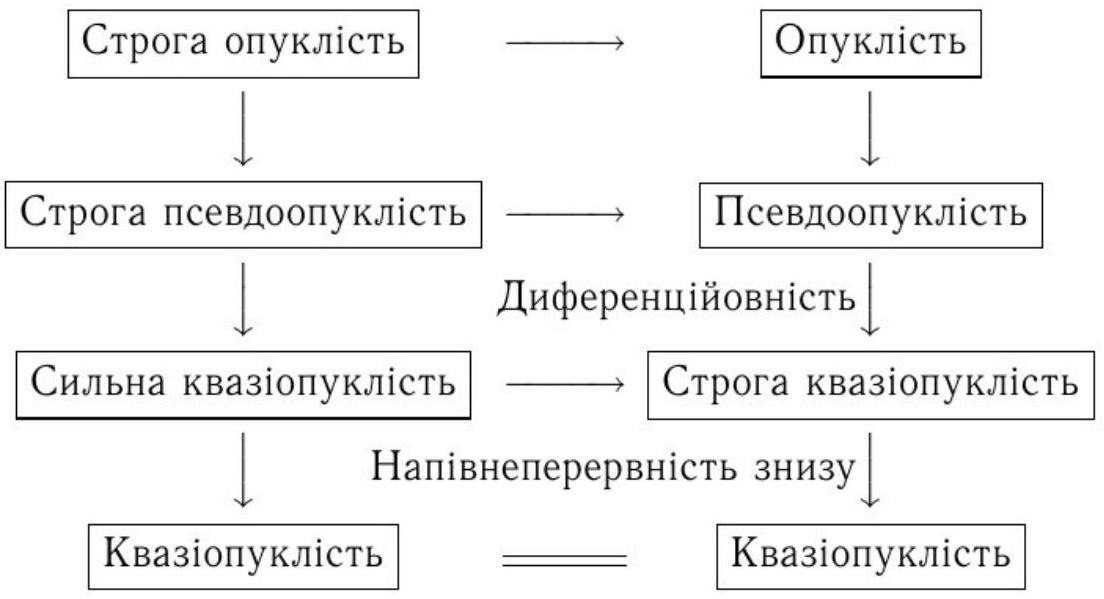
\includegraphics[alt={},max width=\textwidth]{6e2cc08c-e103-486e-965d-56342b3cf45f-3_599_1104_927_274}
\end{center}
\end{figure}

\section*{Похідна за напрямком.}
Похідна функції $f$ у точці $x$ за напрямком $p$ визначається як

$$
f^{\prime}(x, p)=\lim _{\lambda \Downarrow 0} \frac{f(x+\lambda p)-f(x)}{\lambda},
$$

якщо ця границя існує.

\section*{Субградієнт і субдиференціал.}
Вектор $x^{*} \in X^{*}$ називається субградієнтом функції $f$ у точці $x_{0}$, якщо

$$
f(x)-f\left(x_{0}\right) \geq\left\langle x^{*}, x-x_{0}\right\rangle \quad \forall x \in X .
$$

Множина всіх субградієнтів називається субдиференціалом функції $f$ у точці $x_{0}$ і позначається $\partial f\left(x_{0}\right)$.

\section*{Субдиференціал і похідна за напрямком опуклої функції.}
Якщо $f$ - неперервна в точці $x_{0}$ опукла функція, то $\partial f\left(x_{0}\right)$ є непорожньою, замкнутою, опуклою і обмеженою множиною, причому

$$
f^{\prime}\left(x_{0}, p\right)=\max _{x^{*} \in \partial f\left(x_{0}\right)}\left\langle p, x^{*}\right\rangle .
$$

Якщо $f$ диференційовна в точці $x_{0}$, то

$$
\partial f\left(x_{0}\right)=\left\{f^{\prime}\left(x_{0}\right)\right\} .
$$

\section*{Теорема Моро-Рокафеллара.}
Нехай $f_{1}, \ldots, f_{n}$ - власні опуклі функції на $X$. Тоді для кожної точки $x \in X$

$$
\partial f_{1}(x)+\cdots+\partial f_{n}(x) \subset \partial\left(f_{1}+\cdots+f_{n}\right)(x)
$$

Якщо в деякій точці $x_{1} \in\left(\operatorname{dom} f_{1}\right) \cap \cdots \cap\left(\operatorname{dom} f_{n}\right)$ функції $f_{1}(x), \ldots, f_{n}(x)$, за виключенням може однієї, неперервні, то

$$
\partial f_{1}(x)+\cdots+\partial f_{n}(x)=\partial\left(f_{1}+\cdots+f_{n}\right)(x)
$$

для всіх $x \in X$.

\section*{Субдиференціал індикаторної функції.}
Для індикаторної функції $\delta(x \mid M)$ опуклої множини $M$ та точки $x_{0} \in M$ виконується

$$
\partial \delta\left(x_{0} \mid M\right)=-\left(\operatorname{cone}\left(M-x_{0}\right)\right)^{*} .
$$

\section*{Субдиференціал максимуму функцій.}
Нехай $f(x)=\max _{i=1, \ldots, m} f_{i}(x)$, де $f_{i}$ опуклі і неперервні в точці $x_{0}$. Тоді

$$
\partial f\left(x_{0}\right)=\operatorname{conv}\left(\bigcup_{i \in I\left(x_{0}\right)} \partial f_{i}\left(x_{0}\right)\right),
$$

де

$$
I\left(x_{0}\right)=\left\{i: f_{i}\left(x_{0}\right)=f\left(x_{0}\right)\right\} .
$$

\section*{Субдиференціал композиції функцій.}
Нехай $\Lambda: X \rightarrow Y$ - неперервний лінійний оператор, $f$ - опукла функція на $Y$. Тоді для кожної точки $x \in X$ справджується

$$
\Lambda^{*} \partial f(\Lambda x) \subset \partial(f \Lambda)(x)
$$

Якщо функція $f$ неперервна в деякій точці $y_{0} \in \operatorname{Im} \Lambda$, то для кожної точки $x \in X$ справджується рівність

$$
\Lambda^{*} \partial f(\Lambda x)=\partial(f \Lambda)(x)
$$

Нехай $g_{1}, \ldots, g_{m}$ - опуклі функції на $X, g=\left(g_{1}, \ldots, g_{m}\right)$ - утворена з них вектор-функція, $\varphi$ - монотонно неспадна опукла функція на відкритій опуклій множині $U \subset \mathbb{R}^{m}, g(X) \subset U$. Якщо функція $g(x)$ неперервна в точці $x_{0}$, а функція $\varphi$ неперервна в точці $g\left(x_{0}\right)$, то субдиференціал функції $f\left(x_{0}\right)=\varphi\left(g\left(x_{0}\right)\right)$ має вигляд

$$
\partial f\left(x_{0}\right)=\bigcup_{p \in \partial \varphi(u)}\left(\sum_{i=1}^{m} p_{i} \partial g_{i}\left(x_{0}\right)\right),
$$

де $u=g\left(x_{0}\right)$.\\
Зокрема, якщо функція $\varphi$ диференційовна в точці $u=g\left(x_{0}\right)$, то формула матиме вигляд

$$
\partial f\left(x_{0}\right)=\sum_{i=1}^{m} \frac{\partial \varphi}{\partial u_{i}}\left(g\left(x_{0}\right)\right) \partial g_{i}\left(x_{0}\right) .
$$

Якщо, крім того, функції $g_{1}, \ldots, g_{m}$ диференційовні в точці $x_{0}$, то отримаємо відому формулу для градієнта суперпозиції диференційовних функцій:

$$
f^{\prime}\left(x_{0}\right)=\sum_{i=1}^{m} \frac{\partial \varphi}{\partial u_{i}}\left(g\left(x_{0}\right)\right) g_{i}^{\prime}\left(x_{0}\right) .
$$

Функція відстані до множини.\\
Нехай $M$ - опукла множина, $C$ - опукла, обмежена множина, $0 \in \operatorname{int} C$. Тоді для всіх $x \in X$ визначена функція

$$
d_{C}(x \mid M)=\inf _{\rho}\{\rho \geq 0: x \in M+\rho C\}
$$

Якщо $C=B$, де $B$ - одинична куля з центром в нулі, то $d_{B}(x \mid M)$ - це відстань від точки $x$ до множини $M$. Якщо $M=\{0\}$, то

$$
d_{C}(x \mid\{0\})=\inf _{\rho}\{(\rho>0: x \in \rho C)\}=\inf _{\rho}\left\{\left(\rho>0: \frac{x}{\rho} \in C\right)\right\}=\mu(x \mid C),
$$

де $\mu(x \mid C)$ - функція Мінковського.

\section*{Розділ III. Верхня опукла апроксимація}
\section*{Конус дотичних напрямків.}
Конус дотичних напрямків описує ті напрямки, у яких можна локально рухатися від точки множини з малою поправкою.

Вектор $g \in X$ називається дотичним до множини $M$ в точці $x \in M$, якщо існує така функція $\varphi(\lambda) \in X$, що

$$
x+\lambda g+\varphi(\lambda) \in M
$$

при достатньо малих $\lambda \geq 0$ і $\lambda^{-1} \varphi(\lambda) \rightarrow 0$ коли $\lambda \downarrow 0$.\\
Дотичні напрямки утворюють деякі множини - як правило конуси: якщо $g$ - дотичний вектор, то і вектор $\alpha g, \alpha \geq 0$, теж є дотичним.\\
Опуклий конус $K(x, M)$ називається конусом дотичних напрямків до множини $M$ в точці $x$, якщо з включення $g \in K(x, M)$ випливає, що $g$ - дотичний вектор до множини $M$ в точці $x \in M$.

Якщо $M$ - опукла множина, то

$$
K(x, M)=\operatorname{cone}(M-x)=\{g: g=\lambda(y-x), y \in M, \lambda>0\}
$$

є конусом дотичних напрямків до $M$. Для цього достатньо покласти $\varphi(\lambda) \equiv 0$ в означенні.

\section*{Шатра.}
Конус дотичних напрямків містить напрямки, для кожного з яких в означенні існує своя функція $\varphi(\lambda)$. Цього виявляеться недостатньо для того, щоб робити висновки про властивості множини $M$.

Конус дотичних напрямків $K\left(x_{0}, M\right)$ в точці $x_{0} \in M$ називається локальним шатром, якщо для кожного напрямку $g \in \operatorname{ri} K\left(x_{0}, M\right)$ існує опуклий конус $Q$ і визначене в околі початку координат неперервне відображення $\psi(g)$ такі, що:

$$
\begin{aligned}
& \text { а) } \quad g \in \operatorname{ri} Q, \quad \operatorname{Lin} Q=\operatorname{Lin} K\left(x_{0}, M\right), \quad Q \subseteq K\left(x_{0}, M\right) ; \\
& \text { б) } \psi(g)=g+r(g), \quad\|g\|^{-1} r(g) \rightarrow 0 \quad \text { при } g \rightarrow 0 ; \\
& \text { в) } \quad x_{0}+\psi(g) \in M \quad \text { для } g \in Q \cap(\varepsilon B) \quad \text { при деякому } \varepsilon>0 .
\end{aligned}
$$

$B$ - одинична куля в просторі $X=\mathbb{R}^{n}$.


\end{document}